% Auto-generated from docs/schematic/spec_bio.py via render.py — edit the template, not the .tex.
\documentclass[tikz,border=6pt]{standalone}
\usepackage{amsmath}
\usepackage{tikz}
\usetikzlibrary{arrows.meta,calc}
\definecolor{predcolor}{HTML}{4C8DFF}
\definecolor{errcolor}{HTML}{E0772B}
\definecolor{regionstroke}{HTML}{222222}
\definecolor{relaystroke}{HTML}{888888}
\definecolor{interfill}{HTML}{6E6E6E}
\definecolor{rulecol}{HTML}{C9C9C9}
\definecolor{titlecol}{HTML}{222222}
\begin{document}
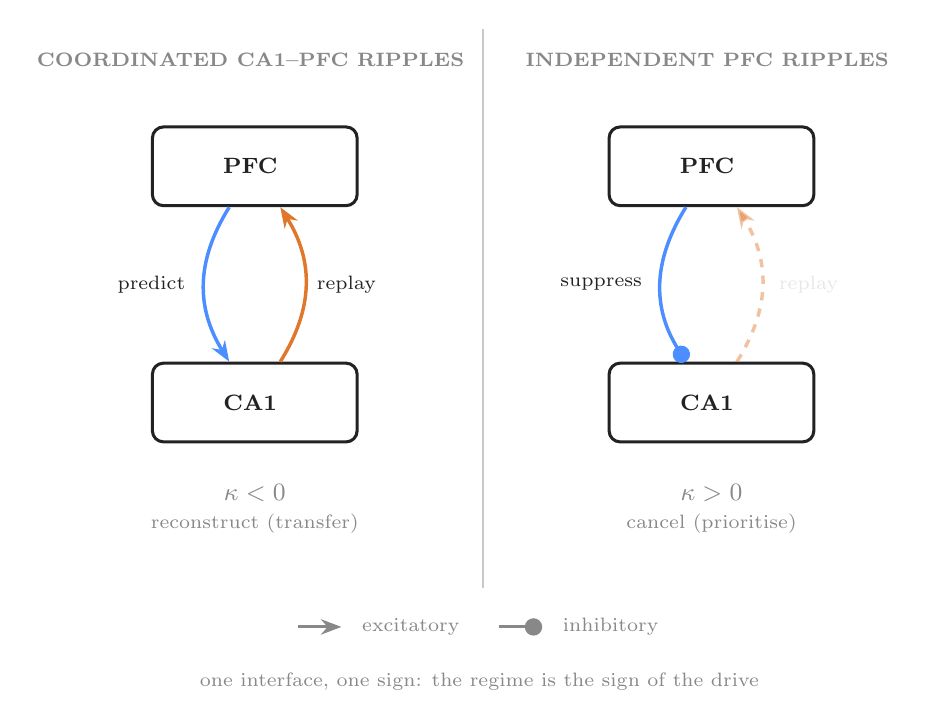
\begin{tikzpicture}[
  % --- nodes ---
  region/.style={rounded corners=4pt, draw=regionstroke, line width=1.1pt, fill=white,
                 align=center, inner sep=3pt, text=titlecol},
  relay/.style={rounded corners=3pt, draw=relaystroke, line width=0.9pt, fill=white,
                align=center, inner sep=3pt, text=titlecol},
  inter/.style={circle, draw=interfill, fill=interfill, minimum size=3.4mm, inner sep=0pt},
  value/.style={circle, draw=regionstroke, line width=1.1pt, fill=white,
                align=center, inner sep=0pt, text=titlecol},
  err/.style={rounded corners=3pt, draw=relaystroke, dashed, line width=0.9pt, fill=white,
              align=center, inner sep=2pt, text=titlecol},
  ghost/.style={inner sep=0pt, minimum size=0pt},
  % --- couplings: colour = direction, terminal = sign ---
  down/.style={predcolor, line width=1.25pt},
  up/.style={errcolor, line width=1.25pt},
  local/.style={relaystroke, line width=1.1pt},
  corr/.style={relaystroke!75, line width=0.7pt, dotted},
  excit/.style={-{Stealth[length=2.6mm]}},
  inhib/.style={-{Circle[length=2.2mm, width=2.2mm]}},
  selfloop/.style={-{Stealth[length=2.2mm]}, relaystroke, line width=0.9pt, looseness=11},
  % --- lettering ---
  glab/.style={font=\scriptsize, fill=white, inner sep=1.5pt, align=center, text=titlecol},
  note/.style={font=\scriptsize, text=relaystroke, align=center},
  panel/.style={font=\scriptsize\bfseries, text=relaystroke, align=center},
  lgd/.style={font=\scriptsize, text=relaystroke},
]
% ---- regions, relays, interneurons ----
\node[region, minimum width=2.60cm, minimum height=1.00cm] (pfc1) at (0.00,-0.00) { { \footnotesize\bfseries PFC } };
\node[region, minimum width=2.60cm, minimum height=1.00cm] (hpc1) at (0.00,-3.00) { { \footnotesize\bfseries CA1 } };
\node[region, minimum width=2.60cm, minimum height=1.00cm] (pfc2) at (5.80,-0.00) { { \footnotesize\bfseries PFC } };
\node[region, minimum width=2.60cm, minimum height=1.00cm] (hpc2) at (5.80,-3.00) { { \footnotesize\bfseries CA1 } };

% ---- recurrent self-loops ----

% ---- projections ----
\draw[up, excit] (hpc1) to[out=58, in=-58, looseness=1.05] node[glab, pos=0.5, anchor=west, xshift=2pt]{ replay } (pfc1);
\draw[down, excit] (pfc1) to[out=-122, in=122, looseness=1.05] node[glab, pos=0.5, anchor=east, xshift=-2pt]{ predict } (hpc1);
\draw[up, excit, dashed, opacity=0.45] (hpc2) to[out=58, in=-58, looseness=1.05] node[glab, pos=0.5, anchor=west, xshift=4pt, fill=none]{ {\color{rulecol}replay} } (pfc2);
\draw[down, inhib] (pfc2) to[out=-122, in=122, looseness=1.05] node[glab, pos=0.5, anchor=east, xshift=-2pt]{ suppress } (hpc2);

% ---- panel rules ----
\draw[rulecol, line width=0.6pt] (2.90,1.75) -- (2.90,-5.35);

% ---- captions ----
\node[panel, anchor=center] at (0.00,1.35) { COORDINATED CA1--PFC RIPPLES };
\node[panel, anchor=center] at (5.80,1.35) { INDEPENDENT PFC RIPPLES };
\node[note, anchor=center] at (0.00,-4.35) { {\small$\kappa<0$}\\[2pt]reconstruct (transfer) };
\node[note, anchor=center] at (5.80,-4.35) { {\small$\kappa>0$}\\[2pt]cancel (prioritise) };
\node[note, anchor=center] at (2.90,-6.55) { one interface, one sign: the regime is the sign of the drive };

% ---- legend: arrowhead = excitatory, dot = inhibitory ----
\draw[local, excit, line width=1.1pt] (0.55,-5.85) -- ++(0.55,0);
\node[lgd, anchor=west] at (1.24,-5.85) { excitatory };
\draw[local, inhib, line width=1.1pt] (3.10,-5.85) -- ++(0.55,0);
\node[lgd, anchor=west] at (3.79,-5.85) { inhibitory };

\end{tikzpicture}
\end{document}